% Created by tikzDevice version 0.12.6 on 2024-04-16 16:18:12
% !TEX encoding = UTF-8 Unicode
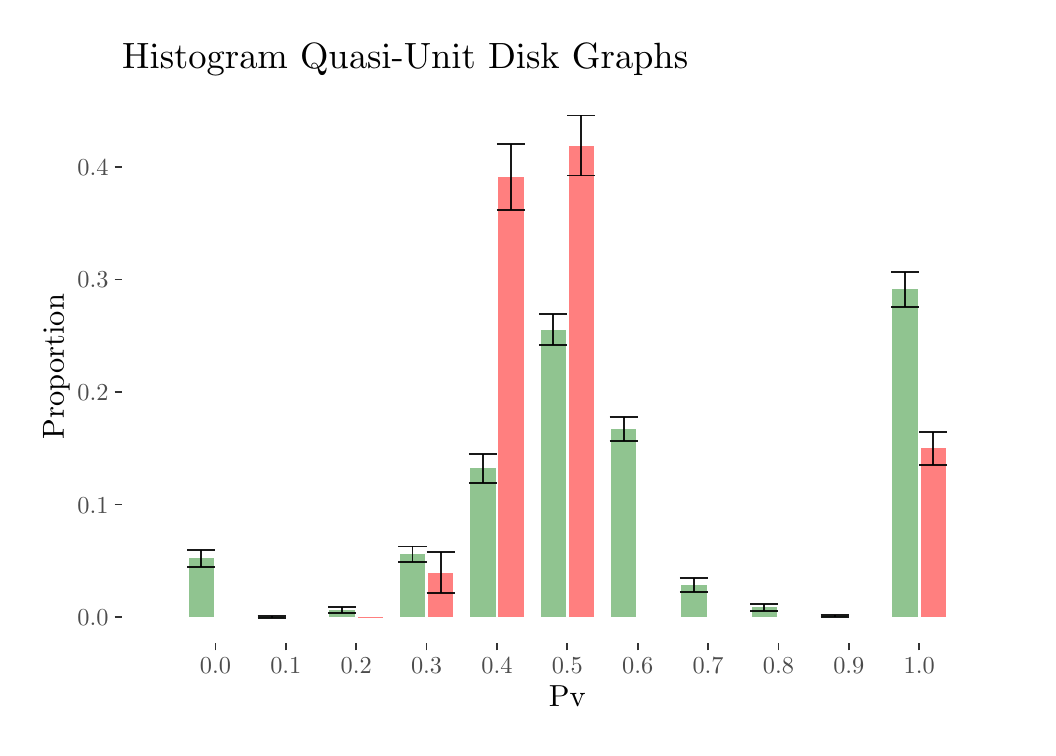
\begin{tikzpicture}[x=1pt,y=1pt]
\definecolor{fillColor}{RGB}{255,255,255}
\path[use as bounding box,fill=fillColor,fill opacity=0.00] (0,0) rectangle (361.35,252.94);
\begin{scope}
\path[clip] (  0.00,  0.00) rectangle (361.35,252.94);
\definecolor{drawColor}{RGB}{255,255,255}
\definecolor{fillColor}{RGB}{255,255,255}

\path[draw=drawColor,line width= 0.6pt,line join=round,line cap=round,fill=fillColor] (  0.00,  0.00) rectangle (361.35,252.94);
\end{scope}
\begin{scope}
\path[clip] ( 34.16, 30.69) rectangle (355.85,230.29);
\definecolor{fillColor}{RGB}{255,255,255}

\path[fill=fillColor] ( 34.16, 30.69) rectangle (355.85,230.29);
\definecolor{fillColor}{RGB}{34,139,34}

\path[fill=fillColor,fill opacity=0.50] ( 58.19, 39.90) rectangle ( 67.34, 61.24);

\path[fill=fillColor,fill opacity=0.50] ( 83.62, 39.90) rectangle ( 92.77, 40.05);

\path[fill=fillColor,fill opacity=0.50] (109.05, 39.90) rectangle (118.20, 42.66);

\path[fill=fillColor,fill opacity=0.50] (134.48, 39.90) rectangle (143.63, 62.64);

\path[fill=fillColor,fill opacity=0.50] (159.91, 39.90) rectangle (169.06, 93.66);

\path[fill=fillColor,fill opacity=0.50] (185.34, 39.90) rectangle (194.49,143.76);

\path[fill=fillColor,fill opacity=0.50] (210.77, 39.90) rectangle (219.92,107.97);

\path[fill=fillColor,fill opacity=0.50] (236.20, 39.90) rectangle (245.36, 51.59);

\path[fill=fillColor,fill opacity=0.50] (261.63, 39.90) rectangle (270.79, 43.45);

\path[fill=fillColor,fill opacity=0.50] (287.06, 39.90) rectangle (296.22, 40.30);

\path[fill=fillColor,fill opacity=0.50] (312.49, 39.90) rectangle (321.65,158.37);
\definecolor{fillColor}{RGB}{255,0,0}

\path[fill=fillColor,fill opacity=0.50] (119.22, 39.90) rectangle (128.38, 39.92);

\path[fill=fillColor,fill opacity=0.50] (144.65, 39.90) rectangle (153.81, 56.04);

\path[fill=fillColor,fill opacity=0.50] (170.08, 39.90) rectangle (179.24,199.08);

\path[fill=fillColor,fill opacity=0.50] (195.51, 39.90) rectangle (204.67,210.36);

\path[fill=fillColor,fill opacity=0.50] (322.66, 39.90) rectangle (331.82,100.90);
\definecolor{drawColor}{RGB}{0,0,0}

\path[draw=drawColor,draw opacity=0.90,line width= 0.7pt,line join=round] ( 57.68, 64.28) --
	( 67.85, 64.28);

\path[draw=drawColor,draw opacity=0.90,line width= 0.7pt,line join=round] ( 62.77, 64.28) --
	( 62.77, 58.21);

\path[draw=drawColor,draw opacity=0.90,line width= 0.7pt,line join=round] ( 57.68, 58.21) --
	( 67.85, 58.21);

\path[draw=drawColor,draw opacity=0.90,line width= 0.7pt,line join=round] ( 83.11, 40.34) --
	( 93.28, 40.34);

\path[draw=drawColor,draw opacity=0.90,line width= 0.7pt,line join=round] ( 88.20, 40.34) --
	( 88.20, 39.76);

\path[draw=drawColor,draw opacity=0.90,line width= 0.7pt,line join=round] ( 83.11, 39.76) --
	( 93.28, 39.76);

\path[draw=drawColor,draw opacity=0.90,line width= 0.7pt,line join=round] (108.54, 43.75) --
	(118.71, 43.75);

\path[draw=drawColor,draw opacity=0.90,line width= 0.7pt,line join=round] (113.63, 43.75) --
	(113.63, 41.57);

\path[draw=drawColor,draw opacity=0.90,line width= 0.7pt,line join=round] (108.54, 41.57) --
	(118.71, 41.57);

\path[draw=drawColor,draw opacity=0.90,line width= 0.7pt,line join=round] (133.97, 65.47) --
	(144.14, 65.47);

\path[draw=drawColor,draw opacity=0.90,line width= 0.7pt,line join=round] (139.06, 65.47) --
	(139.06, 59.82);

\path[draw=drawColor,draw opacity=0.90,line width= 0.7pt,line join=round] (133.97, 59.82) --
	(144.14, 59.82);

\path[draw=drawColor,draw opacity=0.90,line width= 0.7pt,line join=round] (159.40, 98.85) --
	(169.57, 98.85);

\path[draw=drawColor,draw opacity=0.90,line width= 0.7pt,line join=round] (164.49, 98.85) --
	(164.49, 88.47);

\path[draw=drawColor,draw opacity=0.90,line width= 0.7pt,line join=round] (159.40, 88.47) --
	(169.57, 88.47);

\path[draw=drawColor,draw opacity=0.90,line width= 0.7pt,line join=round] (184.83,149.41) --
	(195.00,149.41);

\path[draw=drawColor,draw opacity=0.90,line width= 0.7pt,line join=round] (189.92,149.41) --
	(189.92,138.11);

\path[draw=drawColor,draw opacity=0.90,line width= 0.7pt,line join=round] (184.83,138.11) --
	(195.00,138.11);

\path[draw=drawColor,draw opacity=0.90,line width= 0.7pt,line join=round] (210.26,112.27) --
	(220.43,112.27);

\path[draw=drawColor,draw opacity=0.90,line width= 0.7pt,line join=round] (215.35,112.27) --
	(215.35,103.67);

\path[draw=drawColor,draw opacity=0.90,line width= 0.7pt,line join=round] (210.26,103.67) --
	(220.43,103.67);

\path[draw=drawColor,draw opacity=0.90,line width= 0.7pt,line join=round] (235.69, 54.12) --
	(245.86, 54.12);

\path[draw=drawColor,draw opacity=0.90,line width= 0.7pt,line join=round] (240.78, 54.12) --
	(240.78, 49.06);

\path[draw=drawColor,draw opacity=0.90,line width= 0.7pt,line join=round] (235.69, 49.06) --
	(245.86, 49.06);

\path[draw=drawColor,draw opacity=0.90,line width= 0.7pt,line join=round] (261.12, 44.70) --
	(271.29, 44.70);

\path[draw=drawColor,draw opacity=0.90,line width= 0.7pt,line join=round] (266.21, 44.70) --
	(266.21, 42.20);

\path[draw=drawColor,draw opacity=0.90,line width= 0.7pt,line join=round] (261.12, 42.20) --
	(271.29, 42.20);

\path[draw=drawColor,draw opacity=0.90,line width= 0.7pt,line join=round] (286.55, 40.68) --
	(296.72, 40.68);

\path[draw=drawColor,draw opacity=0.90,line width= 0.7pt,line join=round] (291.64, 40.68) --
	(291.64, 39.92);

\path[draw=drawColor,draw opacity=0.90,line width= 0.7pt,line join=round] (286.55, 39.92) --
	(296.72, 39.92);

\path[draw=drawColor,draw opacity=0.90,line width= 0.7pt,line join=round] (311.98,164.70) --
	(322.15,164.70);

\path[draw=drawColor,draw opacity=0.90,line width= 0.7pt,line join=round] (317.07,164.70) --
	(317.07,152.04);

\path[draw=drawColor,draw opacity=0.90,line width= 0.7pt,line join=round] (311.98,152.04) --
	(322.15,152.04);

\path[draw=drawColor,draw opacity=0.90,line width= 0.7pt,line join=round] (144.14, 63.49) --
	(154.31, 63.49);

\path[draw=drawColor,draw opacity=0.90,line width= 0.7pt,line join=round] (149.23, 63.49) --
	(149.23, 48.59);

\path[draw=drawColor,draw opacity=0.90,line width= 0.7pt,line join=round] (144.14, 48.59) --
	(154.31, 48.59);

\path[draw=drawColor,draw opacity=0.90,line width= 0.7pt,line join=round] (169.57,211.06) --
	(179.74,211.06);

\path[draw=drawColor,draw opacity=0.90,line width= 0.7pt,line join=round] (174.66,211.06) --
	(174.66,187.11);

\path[draw=drawColor,draw opacity=0.90,line width= 0.7pt,line join=round] (169.57,187.11) --
	(179.74,187.11);

\path[draw=drawColor,draw opacity=0.90,line width= 0.7pt,line join=round] (195.00,221.21) --
	(205.18,221.21);

\path[draw=drawColor,draw opacity=0.90,line width= 0.7pt,line join=round] (200.09,221.21) --
	(200.09,199.51);

\path[draw=drawColor,draw opacity=0.90,line width= 0.7pt,line join=round] (195.00,199.51) --
	(205.18,199.51);

\path[draw=drawColor,draw opacity=0.90,line width= 0.7pt,line join=round] (322.15,106.78) --
	(332.33,106.78);

\path[draw=drawColor,draw opacity=0.90,line width= 0.7pt,line join=round] (327.24,106.78) --
	(327.24, 95.02);

\path[draw=drawColor,draw opacity=0.90,line width= 0.7pt,line join=round] (322.15, 95.02) --
	(332.33, 95.02);
\end{scope}
\begin{scope}
\path[clip] (  0.00,  0.00) rectangle (361.35,252.94);
\definecolor{drawColor}{gray}{0.30}

\node[text=drawColor,anchor=base east,inner sep=0pt, outer sep=0pt, scale=  0.88] at ( 29.21, 36.87) {0.0};

\node[text=drawColor,anchor=base east,inner sep=0pt, outer sep=0pt, scale=  0.88] at ( 29.21, 77.55) {0.1};

\node[text=drawColor,anchor=base east,inner sep=0pt, outer sep=0pt, scale=  0.88] at ( 29.21,118.23) {0.2};

\node[text=drawColor,anchor=base east,inner sep=0pt, outer sep=0pt, scale=  0.88] at ( 29.21,158.91) {0.3};

\node[text=drawColor,anchor=base east,inner sep=0pt, outer sep=0pt, scale=  0.88] at ( 29.21,199.60) {0.4};
\end{scope}
\begin{scope}
\path[clip] (  0.00,  0.00) rectangle (361.35,252.94);
\definecolor{drawColor}{gray}{0.20}

\path[draw=drawColor,line width= 0.6pt,line join=round] ( 31.41, 39.90) --
	( 34.16, 39.90);

\path[draw=drawColor,line width= 0.6pt,line join=round] ( 31.41, 80.58) --
	( 34.16, 80.58);

\path[draw=drawColor,line width= 0.6pt,line join=round] ( 31.41,121.26) --
	( 34.16,121.26);

\path[draw=drawColor,line width= 0.6pt,line join=round] ( 31.41,161.94) --
	( 34.16,161.94);

\path[draw=drawColor,line width= 0.6pt,line join=round] ( 31.41,202.63) --
	( 34.16,202.63);
\end{scope}
\begin{scope}
\path[clip] (  0.00,  0.00) rectangle (361.35,252.94);
\definecolor{drawColor}{gray}{0.20}

\path[draw=drawColor,line width= 0.6pt,line join=round] ( 67.85, 27.94) --
	( 67.85, 30.69);

\path[draw=drawColor,line width= 0.6pt,line join=round] ( 93.28, 27.94) --
	( 93.28, 30.69);

\path[draw=drawColor,line width= 0.6pt,line join=round] (118.71, 27.94) --
	(118.71, 30.69);

\path[draw=drawColor,line width= 0.6pt,line join=round] (144.14, 27.94) --
	(144.14, 30.69);

\path[draw=drawColor,line width= 0.6pt,line join=round] (169.57, 27.94) --
	(169.57, 30.69);

\path[draw=drawColor,line width= 0.6pt,line join=round] (195.00, 27.94) --
	(195.00, 30.69);

\path[draw=drawColor,line width= 0.6pt,line join=round] (220.43, 27.94) --
	(220.43, 30.69);

\path[draw=drawColor,line width= 0.6pt,line join=round] (245.86, 27.94) --
	(245.86, 30.69);

\path[draw=drawColor,line width= 0.6pt,line join=round] (271.29, 27.94) --
	(271.29, 30.69);

\path[draw=drawColor,line width= 0.6pt,line join=round] (296.72, 27.94) --
	(296.72, 30.69);

\path[draw=drawColor,line width= 0.6pt,line join=round] (322.15, 27.94) --
	(322.15, 30.69);
\end{scope}
\begin{scope}
\path[clip] (  0.00,  0.00) rectangle (361.35,252.94);
\definecolor{drawColor}{gray}{0.30}

\node[text=drawColor,anchor=base,inner sep=0pt, outer sep=0pt, scale=  0.88] at ( 67.85, 19.68) {0.0};

\node[text=drawColor,anchor=base,inner sep=0pt, outer sep=0pt, scale=  0.88] at ( 93.28, 19.68) {0.1};

\node[text=drawColor,anchor=base,inner sep=0pt, outer sep=0pt, scale=  0.88] at (118.71, 19.68) {0.2};

\node[text=drawColor,anchor=base,inner sep=0pt, outer sep=0pt, scale=  0.88] at (144.14, 19.68) {0.3};

\node[text=drawColor,anchor=base,inner sep=0pt, outer sep=0pt, scale=  0.88] at (169.57, 19.68) {0.4};

\node[text=drawColor,anchor=base,inner sep=0pt, outer sep=0pt, scale=  0.88] at (195.00, 19.68) {0.5};

\node[text=drawColor,anchor=base,inner sep=0pt, outer sep=0pt, scale=  0.88] at (220.43, 19.68) {0.6};

\node[text=drawColor,anchor=base,inner sep=0pt, outer sep=0pt, scale=  0.88] at (245.86, 19.68) {0.7};

\node[text=drawColor,anchor=base,inner sep=0pt, outer sep=0pt, scale=  0.88] at (271.29, 19.68) {0.8};

\node[text=drawColor,anchor=base,inner sep=0pt, outer sep=0pt, scale=  0.88] at (296.72, 19.68) {0.9};

\node[text=drawColor,anchor=base,inner sep=0pt, outer sep=0pt, scale=  0.88] at (322.15, 19.68) {1.0};
\end{scope}
\begin{scope}
\path[clip] (  0.00,  0.00) rectangle (361.35,252.94);
\definecolor{drawColor}{RGB}{0,0,0}

\node[text=drawColor,anchor=base,inner sep=0pt, outer sep=0pt, scale=  1.10] at (195.00,  7.64) {Pv};
\end{scope}
\begin{scope}
\path[clip] (  0.00,  0.00) rectangle (361.35,252.94);
\definecolor{drawColor}{RGB}{0,0,0}

\node[text=drawColor,rotate= 90.00,anchor=base,inner sep=0pt, outer sep=0pt, scale=  1.10] at ( 13.08,130.49) {Proportion};
\end{scope}
\begin{scope}
\path[clip] (  0.00,  0.00) rectangle (361.35,252.94);
\definecolor{drawColor}{RGB}{0,0,0}

\node[text=drawColor,anchor=base west,inner sep=0pt, outer sep=0pt, scale=  1.32] at ( 34.16,238.35) {Histogram Quasi-Unit Disk Graphs};
\end{scope}
\end{tikzpicture}
